\chapter{Simulações}

Para que possamos avaliar o efeito que a hiper-racionalidade tem no resultado de um jogo nós iremos simular os mesmos problemas, estruturas e condições iniciais das simulações encontradas em \cite{madeo2015}. A matriz de preferências que usaremos depende do grafo onde a simulação é feita onde as entradas são dadas por
\begin{equation}
    \label{prefComparativo}
    r_{v,u} = \left\{\begin{matrix}
                \frac{1}{2} \text{, se } v=u\\ 
                \frac{1}{2d_v} \text{, se } v\neq u \text{ e } a_{v,u}\neq 0 \\
                 0 \text{, se } a_{v,u}=0
                \end{matrix}\right.,
\end{equation}
onde $d_v$ é o grau do vértice $v$. Em outras palavras, um jogador possui preferência $\frac{1}{2}$ por si e o resto é dividido igualmente entre todos seus vizinhos. As simulações foram feitas para $3$ tipos de grafo estrela em $3$ diferentes condições iniciais para os jogos do dilema do prisioneiro não estrito, biestabilidade e coexistência. As arestas mais grossas na estrela assimétrica ponderada possuem peso $3$, enquanto todas demais arestas possuem peso $1$. 

Vamos começar com o dilema do prisioneiro não estrito, cuja a única diferença do dilema que vimos até o momento é que as desigualdades em $\eqref{desigualdadePD}$ são não estritas. A matriz de pagamentos usada nas simulações é dada por
\begin{equation}
    \label{pagtoPDComparativo}
    B=
    \begin{bmatrix}
        1 & 0\\ 
        \frac{3}{2} & 0 
    \end{bmatrix}
\end{equation}

Podemos ver na figura \ref{fig:prisoner-control.png} o resultado das simulações. Ao contrário do jogo com jogadores racionais, o $\textit{silêncio}$ é predominante dentre os jogadores hiper-racionais e $\textit{delação}$ aparece somente por conta da centralidade de $1$, que distribui o pagamento da tentação para sua vizinhança por conta das hiperpreferências dos jogadores. Porém, ainda temos um equilíbrio misto na estrela assimétrica ponderada para a condição inicial $a$, que surge por conta do incentivo inicial para que $2$ use $\textit{silêncio}$ que é freado quando $1$ passa a usar exclusivamente $\textit{delação}$.

\begin{figure}[h]
    \caption{Probabilidade do jogador usar \textit{silêncio} no dilema do prisioneiro em diferentes grafos estrela com matriz de pagamentos $\eqref{pagtoPDComparativo}$. Na primeira coluna temos a distribuição de estratégias para $t=0$ e nas demais temos a distribuição para $t=100$ nos grafos dados. As simulações para jogadores racionais foram feitas por Madeo e Mocceni e podem ser encontradas em \cite{madeo2015}.}
    \centerline{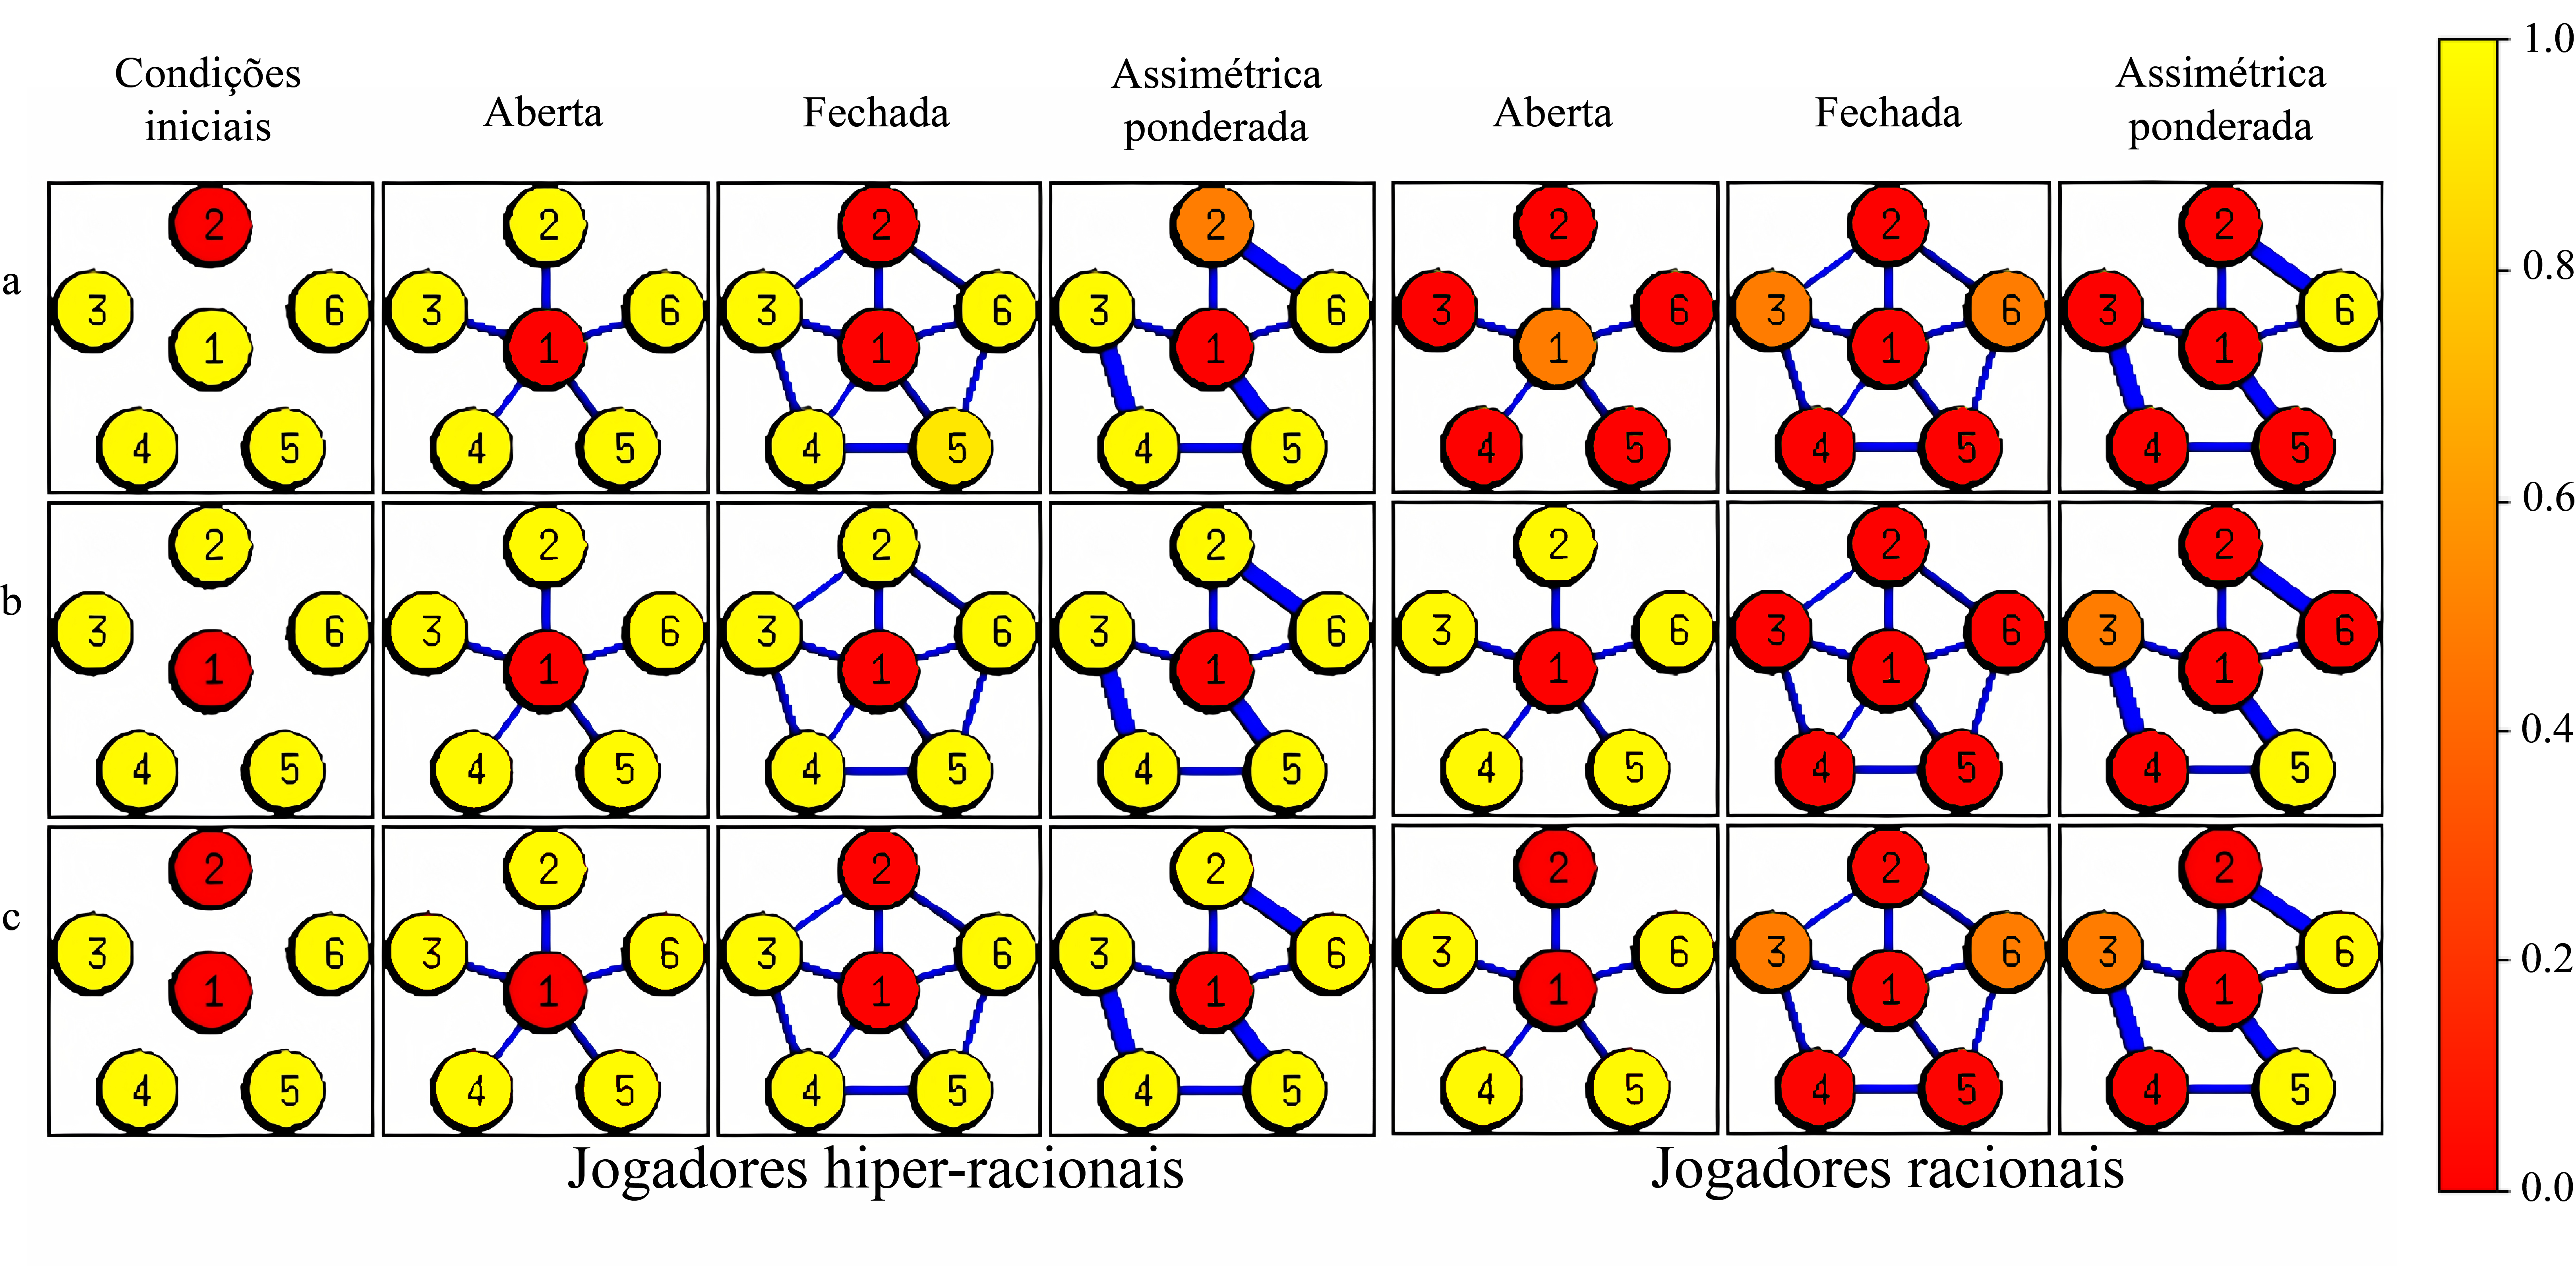
\includegraphics[scale=0.27]{./img/prisoner-control.png}}
    \label{fig:prisoner-control.png}
\end{figure}

No jogo da biestabilidade um jogador recebe um pagamento somente quando joga contra a mesma estratégia que está usando, onde uma delas pode, ou não, gerar um pagamento maior do que a outra. A matriz de pagamentos que foi usada na simulação é a seguinte.
\begin{equation}
    \label{pagtoBiComparativo}
    B=
    \begin{bmatrix}
        1 & 0\\ 
        0 & 1 
    \end{bmatrix}
\end{equation}

O resultado para as simulações do jogo da biestabilidade pode ser observado na figura \ref{fig:bistability-control.png}. Vemos que, no caso racional, os jogadores sempre querem usar a estratégia que a maioria de sua vizinhança usa, o que leva ao equilíbrio misto na estrela aberta com dissidente central e à dissidência de $2$ e $6$ na estrela assimétrica ponderada com condição inicial $c$. No caso hiper-racional temos uma situação parecida, pois as hiperpreferências acentuam o incentivo por estar na moda, fazendo com que não haja mais o equilíbrio misto na estrela aberta e aumentando a importância das relações de menor peso na estrela assimétrica ponderada.

\begin{figure}[h]
    \caption{Probabilidade do jogador usar a estratégia $1$ no jogo da biestabilidade em diferentes grafos estrela com matriz de pagamentos $\eqref{pagtoBiComparativo}$. Na primeira coluna temos a distribuição de estratégias para $t=0$ e nas demais temos a distribuição para $t=50$ nos grafos dados. As simulações para jogadores racionais foram feitas por Madeo e Mocceni e podem ser encontradas em \cite{madeo2015}.}
    \centerline{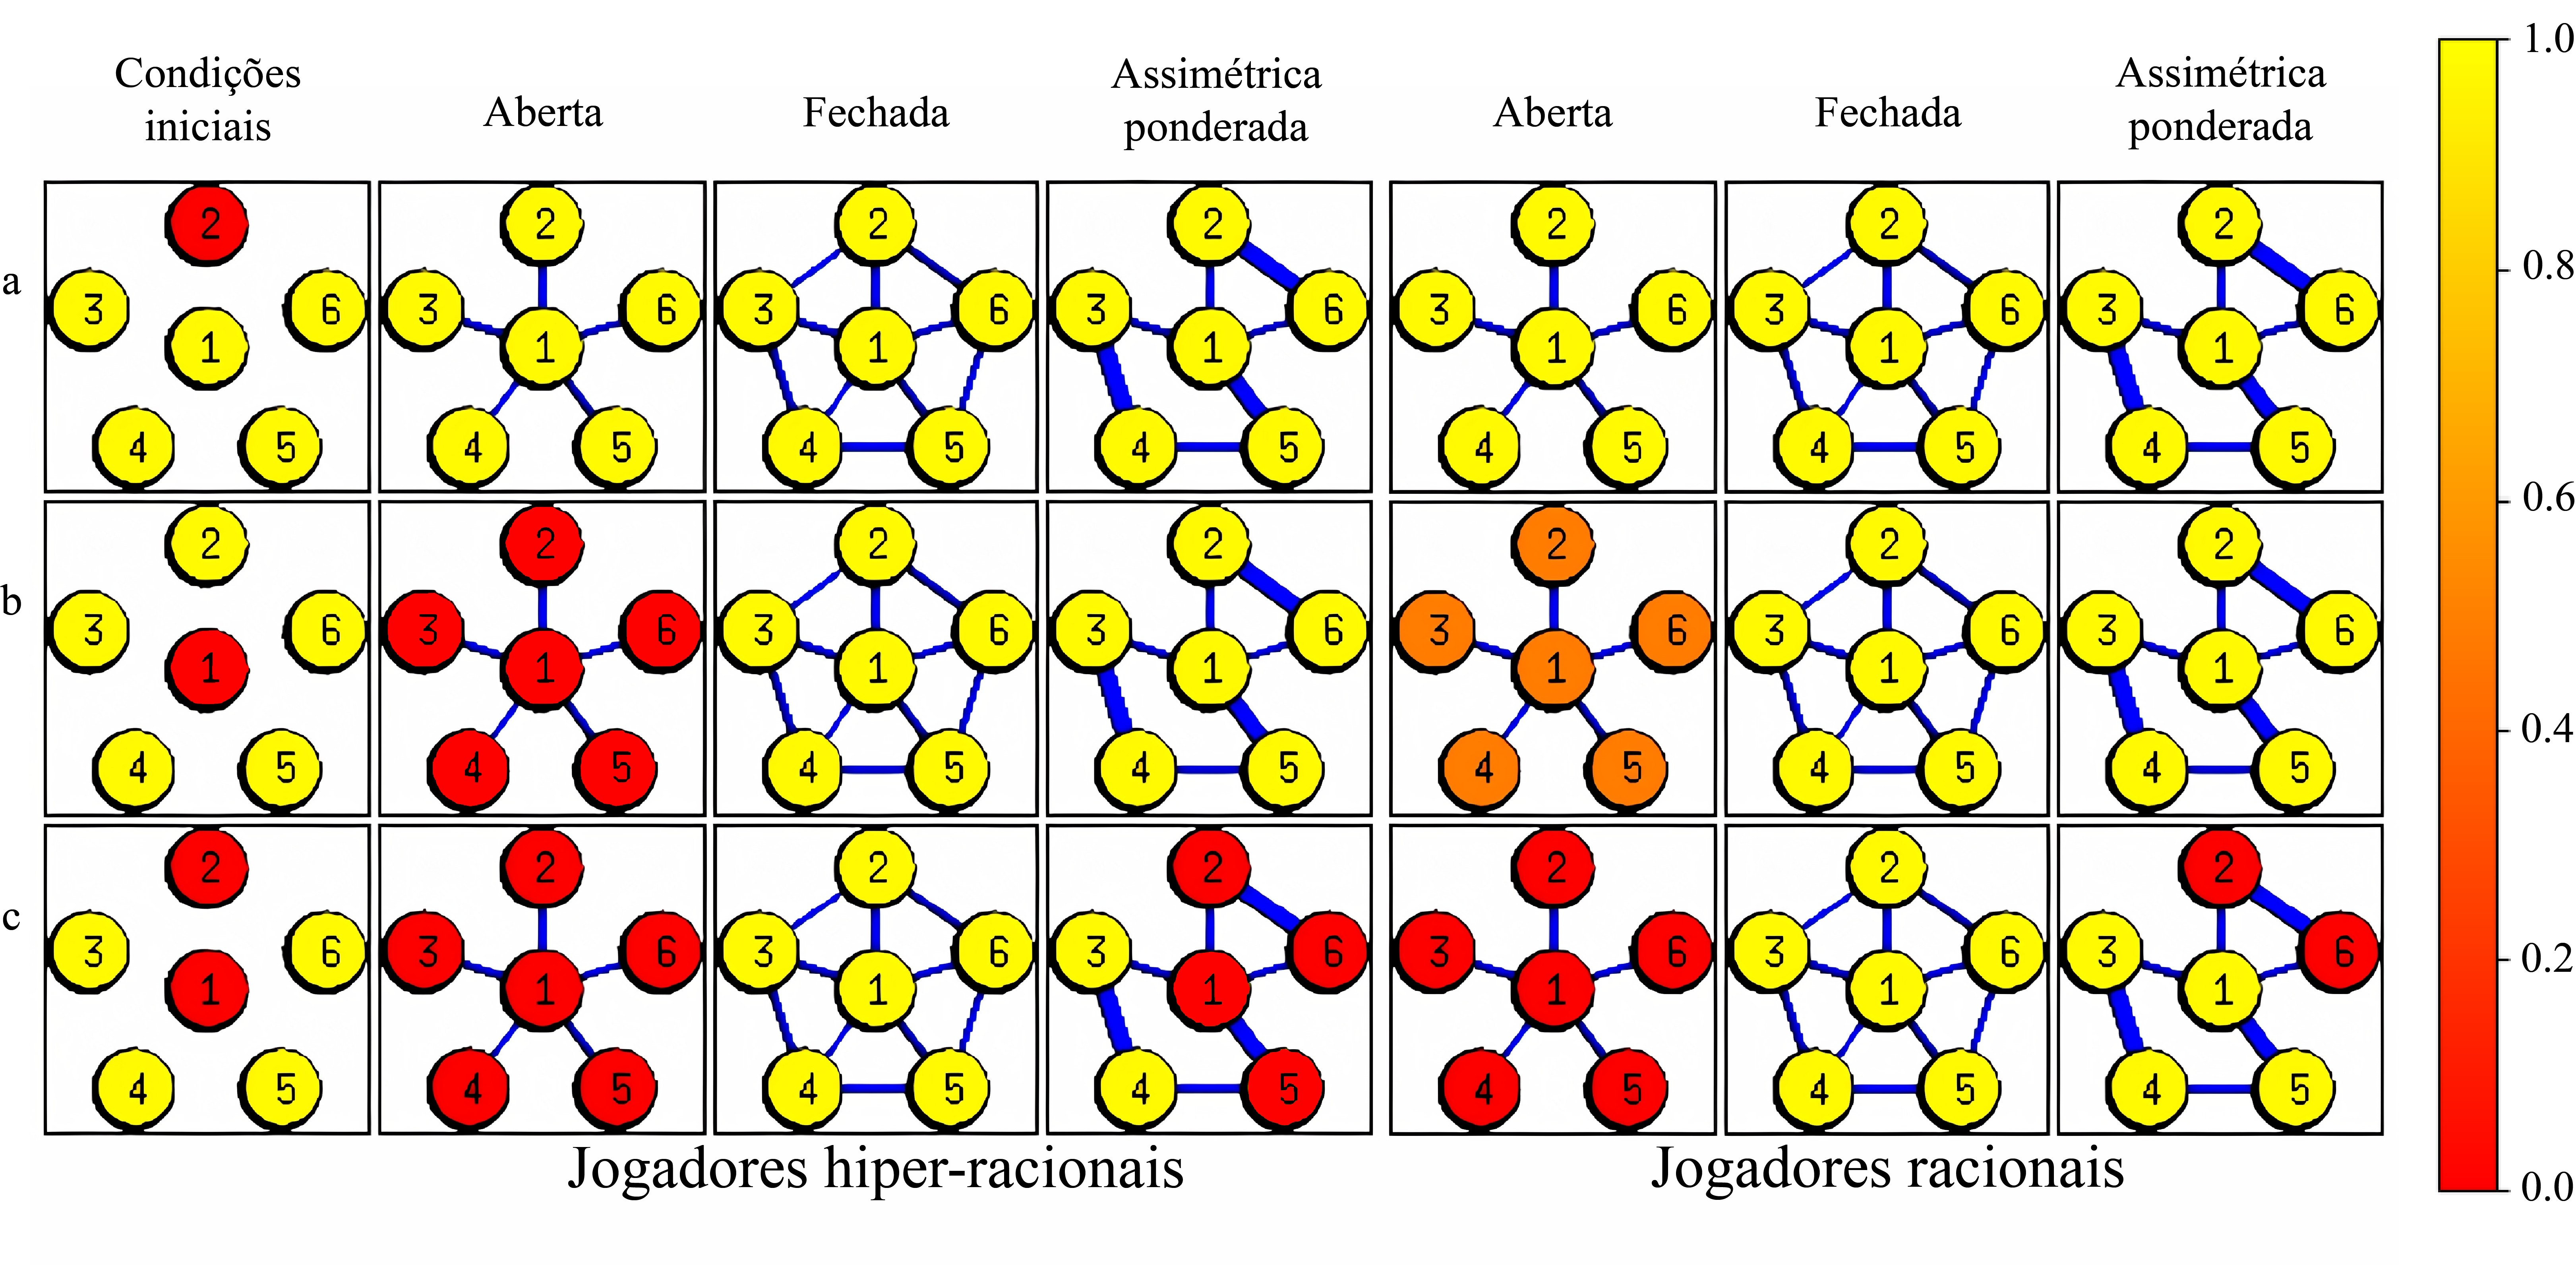
\includegraphics[scale=0.27]{./img/bistability-control.png}}
    \label{fig:bistability-control.png}
\end{figure}

No jogo da coexistência um jogador recebe um pagamento somente quando joga contra uma estratégia diferente da que está usando e todos pagamentos são iguais. A matriz de pagamentos que foi usada na simulação é a seguinte.
\begin{equation}
    \label{pagtoCoexComparativo}
    B=
    \begin{bmatrix}
        0 & 1\\ 
        1 & 0 
    \end{bmatrix}
\end{equation}

O resultado para as simulações do jogo da coexistência pode ser observado na figura \ref{fig:coex-control.png}. Ao contrário da biestabilidade, nesse jogo há um incentivo para ser diferente dos seus vizinhos e podemos ver que os resultados em ambos modelos são praticamente iguais, com exceção dos equilíbrios mistos, que são mais próximos da condição inicial no modelo hiper-racional. Isso se deve às hiperpreferências, que diminuem o incentivo para que os jogadores usem uma estratégia diferente da mais usada em sua vizinhança.

\begin{figure}[h]
    \caption{Probabilidade do jogador usar a estratégia $1$ no jogo da coexistência em diferentes grafos estrela com matriz de pagamentos $\eqref{pagtoCoexComparativo}$. Na primeira coluna temos a distribuição de estratégias para $t=0$ e nas demais temos a distribuição para $t=50$ nos grafos dados. As simulações para jogadores racionais foram feitas por Madeo e Mocceni e podem ser encontradas em \cite{madeo2015}.}
    \centerline{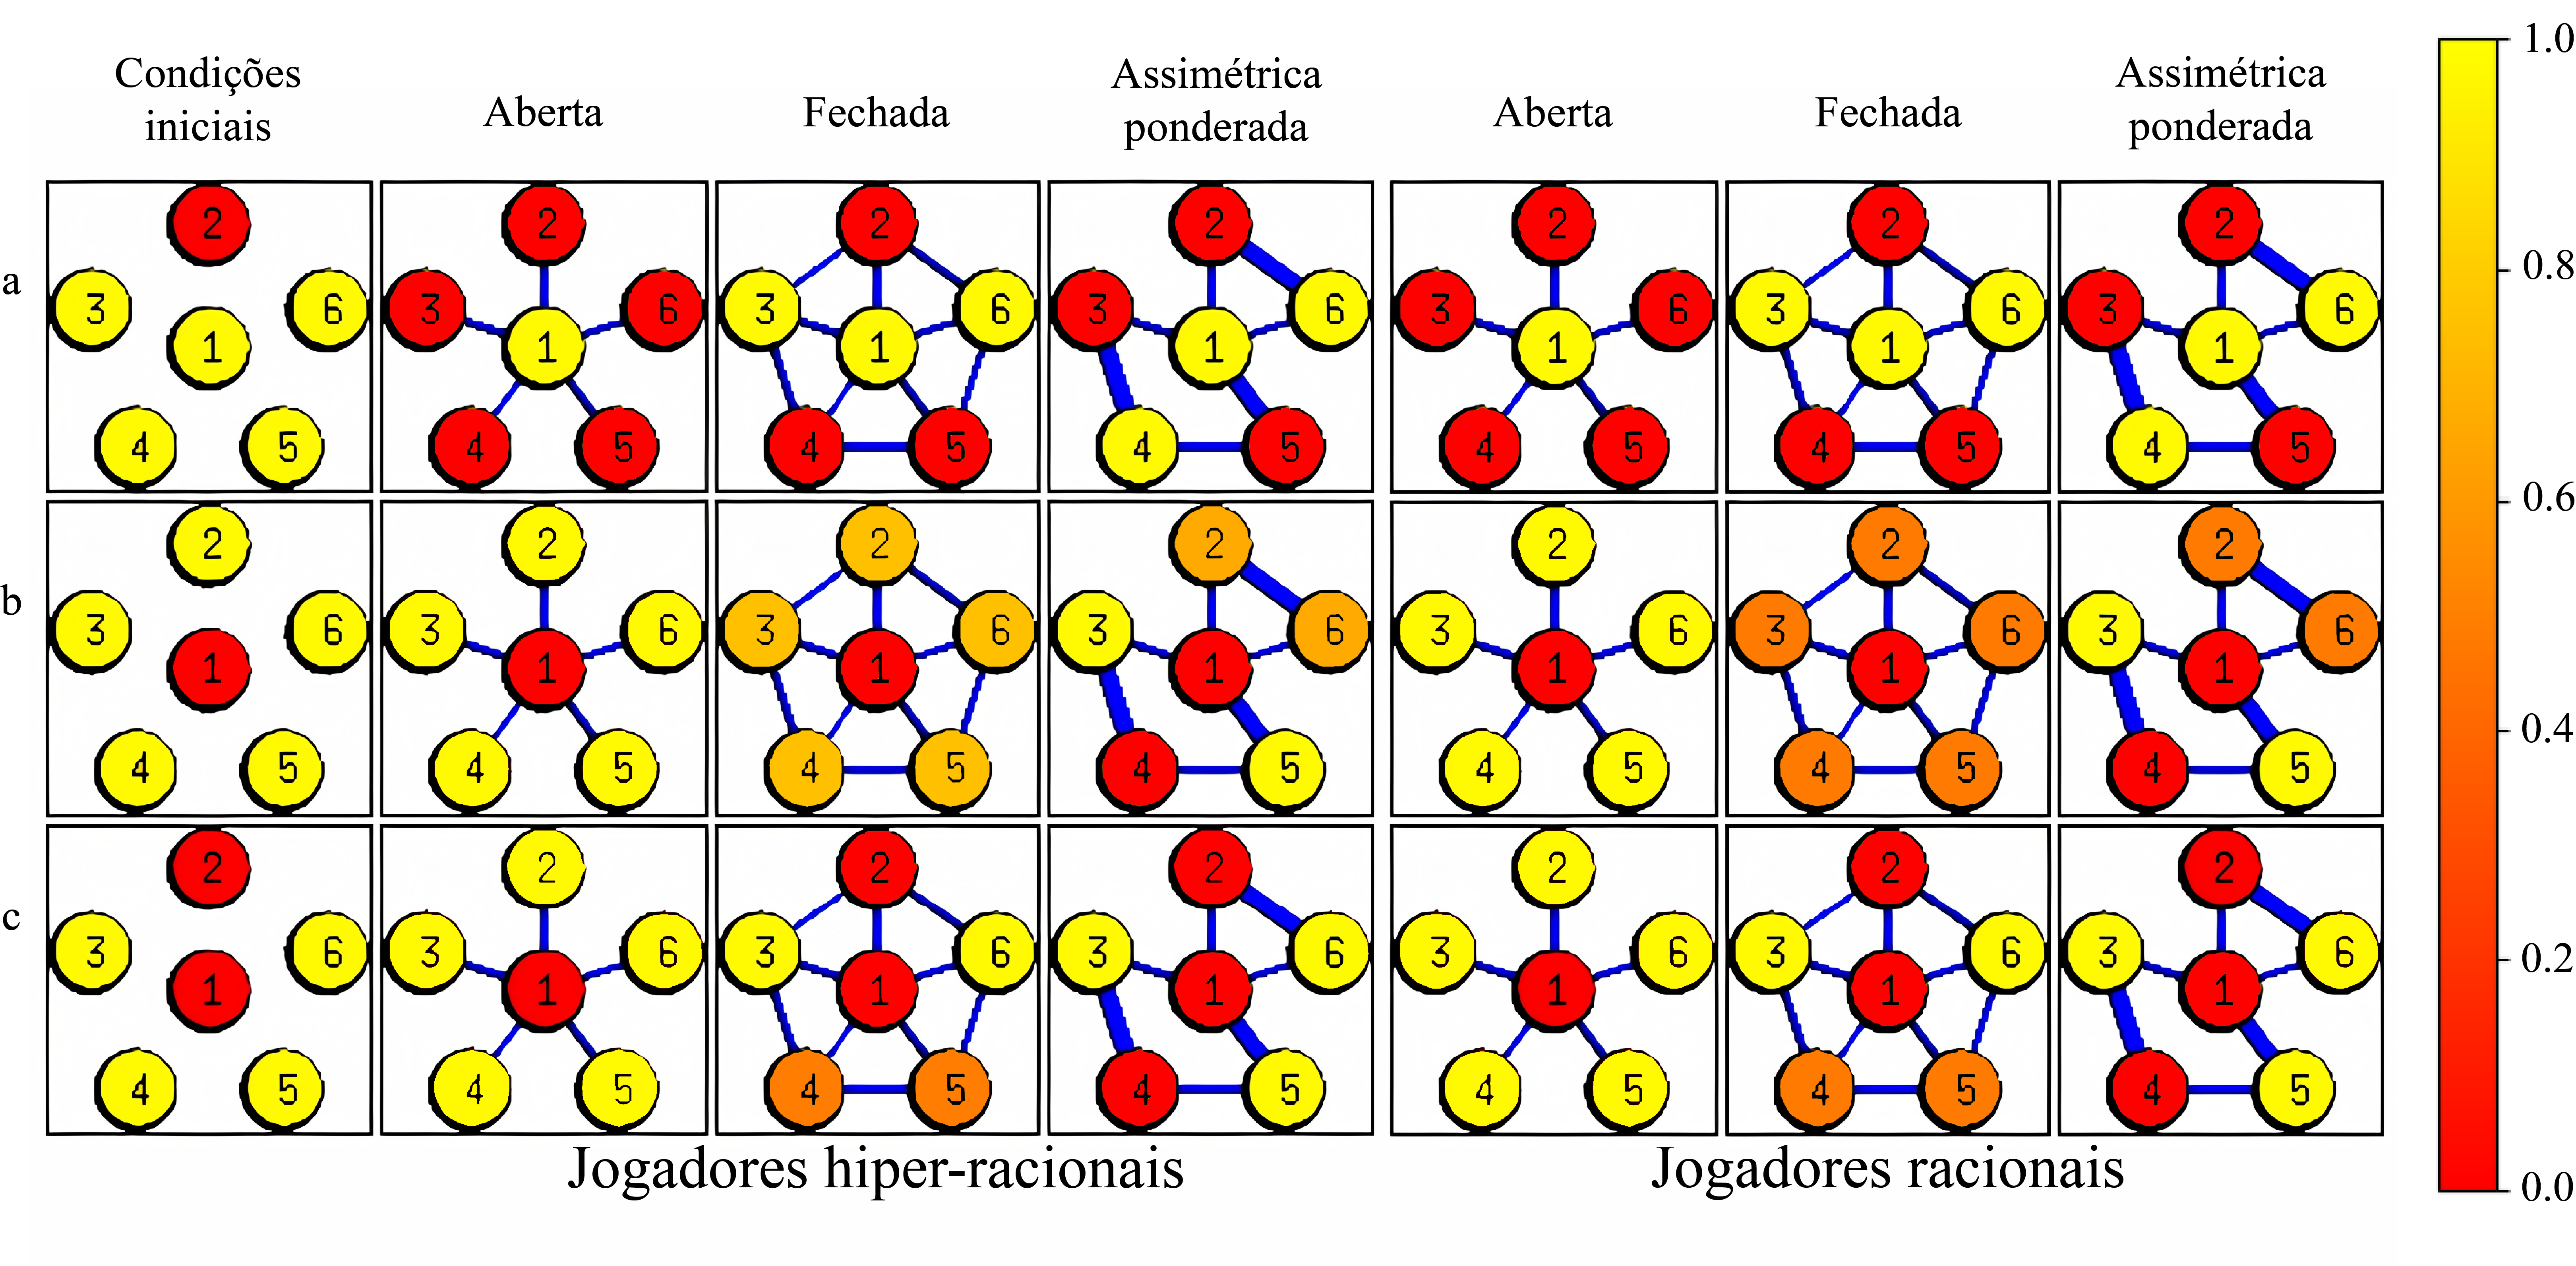
\includegraphics[scale=0.27]{./img/coexistance-control.png}}
    \label{fig:coex-control.png}
\end{figure}

Além de possibilitar uma comparação entre jogadores racionais e hiper-racionais, essas simulações mostram como a estrutura do grafo influencia os hiperequilíbrios do jogo. Vimos que, mesmo para jogadores racionais, os vértices mais centrais exercem maior influência no resultado do jogo, uma característica que é acentuada pelas hiperpreferências positivas, que aumentam o impacto da centralidade no pagamento de todos jogadores.
